\begin{document}


\pagenumbering{gobble}
\newpage
\pagenumbering{arabic}

\noindent(Следовательно, системы со смешанным целочисленным основанием обладают этим свойством. Наиболее общими системами такого типа являются системы со смешанным основанием, у которых $\beta_{1} = (c_{0} + 1)\beta_{0}, \beta_{2} = (c_{1} + 1)(c_{0} + 1)\beta_{0},  \ldots , \beta_{-1} = \beta_{0}/(c_{-1} + 1),  \ldots )$

\paragraph{} \m{21}
Покажите, что любое ненулевое число имеет единственное ''знакопеременное двоичное представление''
\begin{center}
$2^{e_{0}} - 2 ^{e_{1}} +  \ldots  + (-1)^{t}2^{e_{t}}$,
\end{center}
где $e_{0} < e_{1} <  \ldots  < e_{t}$

\paragraphT{} \m{24}
Покажите, что любое неотрицательное комплексное число вида $a + bi$, где $a$ и $b$ — целые числа, обладает единственным ''периодическим двоичным представлением''
\begin{center}
$1+(i)^{e_{0}} + i(1 + i)^{e_{0}} - (1 + i)^{e_{3}} +  \ldots  + i^{-t}(1+i)^{e_{t}}$,
\end{center}
где $e_{0} < e_{1} <  \ldots  < e_{t}$ (ср. с упр. 27).

\paragraph{} \m{35}
(Н. Г. де Брейн (N. G. de Bruijn).) Пусть $S_{0}, S_{1}, S_{2},  \ldots $ - множества неотрицательных целых чисел; говорят, что совокупность $\lbrace S_{0}, S_{1}, S_{2},  \ldots \rbrace$ обладает свойством В, если любое неотрицательное целое число $n$ может быть единственным способом записано в виде
\begin{center}
$n = s_{0} + s_{1} +  \ldots , \tab s_{j} \in S_{j}$
\end{center}
(Свойство В означает, что $0 \in S_{j}$ для всех $j$, поскольку $n = 0$ может быть представлено только как $0 + 0 + 0 +  \ldots $ .) Любая система счисления со смешанным основанием $b_{0}, b_{1}, b_{2}, \ldots $ дает пример совокупности множеств, удовлетворяющих свойству В, если положить $S_{j} = \lbrace 0, B_{j}, \ldots , (b_{j} - 1)B_{j} \rbrace$, где $B_{j} = b_{0}b_{1}  \ldots b_{j-i}.$ В таком случае представление $n = s_{0} + s_{1} + s_{2} +  \ldots  $ очевидным образом соответствует представлению (9) этого числа по смешанному основанию. Далее, если совокупность $\lbrace S_{0}, S_{1}, S_{2}, \ldots \rbrace A_{0}, A_{1}, A_{2},  \ldots $ обладает
свойством В, то, каково бы ни было разбиение $A_{0}, A_{1}, A_{2},  \ldots $ неотрицательных целых чисел (т. е. $A_{0} \cup A_{1} \cup A_{2} U  \ldots  = \lbrace 0,1, 2, \ldots \rbrace$ и $A_{i} \cap A_{j} = \emptyset $ при $ i \neq j $, некоторые из множеств $A_{j}$ могут быть пустыми), этим свойством обладает и полученная из нее путем ''стягивания'' совокупность $\lbrace T_{0}, T_{1}, T_{2}, \ldots  \rbrace$, где множество $T_{j}$ состоит из всех сумм вида $\sum_{i \in A_{j}}s_{i}$ взятых по всевозможным выборкам элементов $s_{i} \in S_{i}$.

Докажите, что любая последовательность $\lbrace T_{0}, T_{1}, T_{2},  \ldots \rbrace$, удовлетворяющая свойству В, может быть получена посредством ''стягивания'' некоторой совокупности $\lbrace S_{0}, S_{1}, S_{2},  \ldots \rbrace$, соответствующей системе счисления по смешанному основанию.

\paragraph{} \m{39}
(Н. Г. де Брейн.) Пример системы счисления по основанию —2 показывает, что любое целое число (положительное, отрицательное или нуль) имеет единственное представление в виде
\begin{center}
$(-2)^{e_{1}} + (-2)^{e_{2}} +  \ldots  + (-2)^{e_{t}}$,\tab $e_{1} >  \ldots  > e_{t} \geq 0$,\tab $t \geq 0$
\end{center}
Назначение данного упражнения - несколько обобщить это свойство.

%Здесь
\begin{enumerate}[label=\alph*)]
\item Пусть последовательность целых чисел $ b_{0}, b_{1}, b_{2},  \ldots $ такова, что любое целое число $ n $ допускает единственное представление в виде
\begin{center}
$ n = b_{e_{1}} + b_{e_{2}} +  \ldots  + b_{e_{t}} $,\tab $ e_{1} > e_{2} >  \ldots  > e_{t} \geq 0 $ ,\tab $ t \geq 0  $. 
\end{center}

(Данная последовательность $\langle b_{n}\rangle $  называется бинарным базисом.) Покажите, что найдется такое значение индекса $j$, что $b_{j}$ нечетно, а для всех $k \neq j$ числа $b_{j}$ четны.

\item Докажите, что бинарный базис $\langle b_{n}\rangle $  всегда может быть преобразован в последовательность вида $d_{0}, 2d_{1}, 4d_{2},  \ldots  = (2^{n}d_{n})$, где каждое из чисел $d_{k}$ нечетно.

\item Докажите, что если каждое из чисел $d_{0}, d_{1}, d_{2},  \ldots $ из п. (b) равно $\pm 1$, то последовательность $\langle b_{n}\rangle $ образует бинарный базис тогда и только тогда, когда существует бесконечно много $d_{j}$, равных $+1$, и бесконечно много $d_{j}$, равных $-1$.

\item Докажите, что последовательность $7, -13 \cdot 2, 7 \cdot 2^{2}, -13 \cdot 2^{2k+1},  \ldots $ является бинарным базисом, и найдите представление числа $n = 1$.
\end{enumerate}

\paragraphT{} \m{35} Одно обобщение представления чисел в двоичном коде, известное как \textquotedblleft 2-адические числа\textquotedblright, было предложено в работе К. Hensel, Crelle 127 (1904), 51-84. (В действительности К. Гензель предложил $p-адические числа$ для любого простого числа р.) 2-адическое число можно рассматривать как двоичное число
\begin{center}
$u = ( \ldots u_{3}u_{2}u_{1}u_{0}.u_{-1}  \ldots  u_{-n})_{2}$,
\end{center}

представление которого бесконечно продолжается влево и лишь на конечное количество знаков вправо от разделяющей точки. Сложение, вычитание и умножение 2-адических чисел выполняются в соответствии с алгоритмом обычных арифметических операций, которые, в принципе, допускают возможность неограниченного продолжения влево. Например,

\begin{center}
\begin{tabular}{c c c}
$ 7 = ( \ldots 000000000000111)_{2} $ & & $ \frac{1}{7} = ( \ldots 110110110110111)_{2} $\\

$-7 = (111111111111001)_{2}$ & & $- \frac{1}{7} = ( \ldots 001001001001001)_{2}$\\

$\frac{7}{4} = ( \ldots 0000000000001.11)_{2}$ & & $\frac{1}{10} = ( \ldots 110011001100110.1)_{2}$\\

$\sqrt{-7} = ( \ldots 1000000010110101)_{2}$ & или & $( \ldots 011111101001011)_{2}$.
\end{tabular}
\end{center}

Здесь число 7 - обычное число \textquotedblleft семь\textquotedblright в двоичном представлении, а $ -7$ - обратный код, неограниченно продолженный влево. Легко проверить, что обычная процедура сложения двоичных чисел дает $ -7 + 7 = ( \ldots 00000)_{2} = 0$, если ее выполнение продолжать неограниченно долго. Значения $\frac{1}{7}$ и $-\frac{1}{7}$ представляют собой единственные 2-адические числа, которые после формального умножения на 7 дают соответственно $1$ и $-1$. Значения $\frac{7}{4}$ и $\frac{1}{10}$ есть примеры 2-адических чисел, не являющихся 2-адическими \textquotedblleft целыми\textquotedblright, так как они имеют ненулевые биты справа от разделяющей точки. Приведенные два значения $\sqrt{-7}$, получающиеся одно из другого в результате перемены знака, являются единственными 2-адическими числами, которые после формального возведения в квадрат
дают $( \ldots  111111111111001)_{2}$.
\begin{enumerate}[label=\alph*)]
\item Докажите, что любое 2-адическое число и можно разделить на произвольное ненулевое 2-адическое число $v$, чтобы вычислить 2-адическое число $w$, удовлетворяющее равенству $u$ = $vw$.\tabn 

%ЗДЕСЬ%
\noindent(Следовательно, множество 2-адических чисел образует поле; см. раздел 4.6.1.)
\item Докажите, что 2-адическое представление рационального числа $-1/(2n + 1)$, где $n$ — положительное целое число, можно получить следующим образом. Сначала находим обычное двоичное разложение числа $+1/(2n + 1)$, которое имеет вид периодической дроби $(0.\alpha\alpha\alpha. . .)_{2}$ ($\alpha$ - некоторая строка из нулей и единиц). Тогда $(. . .\alpha\alpha\alpha)г$ будет 2-адическим представлением числа $-1/(2n + 1)$.
\item Докажите, что 2-адическое представление числа и периодично (т.е. $u_{N + \lambda} = u_{N}$) для всех больших $N$ при некотором $\lambda \geq 1$) тогда и только тогда, когда $u$ рационально (т. е. $u = m/n$ для некоторых целых чисел чисел $m$ и $n$).
\item Докажите, что если $n$ - целое число, то $\sqrt{n}$ является 2-адическим числом только в том случае, если для некоторого неотрицательного целого числа $n$ оно удовлетворяет условию $n$ $mod$ $2^{2k + 3} $ $=$ $2^{2k}$. (Таким образом, либо $n$ $mod$ $8$ $=$ $1$, либо $n$ $mod$ $32$ $=$ $4$, и т. д.)
\end{enumerate}

\paragraph{} \m{40} (И. 3. Руца (I. Z. Ruzsa).) Сформируйте бесконечно много целых чисел, в троичных представлениях которых используются только нули и единицы, а в четверичном представлении - только нули, единицы и двойки.

\paragraph{} \m{40} (Д. А. Кларнер (D. A. Klarner).) Пусть множество $D$ - произвольное множество целых чисел, $b$- любое положительное целое число, а $k_{n}$-количество различных целых чисел, которые могут быть записаны как $n$-разрядные числа $\langle a_{n - 1}  \ldots  a_{1}a_{0})_{b}$ по основанию $b$ с цифрами $a_{i}$ в $D$. Докажите, что последовательность $\langle k_{n}\rangle$ удовлетворяет линейному рекуррентному соотношению, и поясните, как вычислить производящую функцию $\sum_{n}k_{n}z^{n}$. Проиллюстрируйте разработанный алгоритм, показав, что в случае, когда $b = 3$ и $D = \lbrace-1,0,3\rbrace$, число $k_{n}$ есть число Фибоначчи.

\paragraphT{} \M{22} (Г. В. Райтвайзнер (G. W. Reitwiesner), 1960.) Поясните, как представить заданное целое число $n$ в виде $( \ldots  a_{2}a_{1}a_{0})_{2}$, где каждое из $d_{j}$ есть $-1$, $0$ либо $1$, используя наименьшую ненулевую цифру.
\newpage
\section{АРИФМЕТИКА ЧИСЕЛ С ПЛАВАЮЩЕЙ ТОЧКОЙ}

\large{В этом разделе} рассмотрены основные принципы выполнения арифметических операций над числами с ''плавающей точкой'' и проанализирован внутренний механизм таких вычислений. Вероятно, у многих читателей данная тема не вызовет слишком большого интереса либо потому, что в вычислительных машинах, на которых они работают, имеются встроенные команды операций над числами с плавающей точкой, либо потому, что нужные подпрограммы содержатся в операционной системе. Но не следует считать, что материал этого раздела относится исключительно к компетенции инженеров - конструкторов ЭВМ или узкого круга лиц, которые пишут системные подпрограммы для новых машин. Каждый грамотный программист должен иметь представление о том, что происходит при выполнении элементарных шагов арифметических операций над числами с плавающей точкой. Предмет этот совсем не так тривиален, как принято считать; в нем удивительно много интересного.
\subsection{Вычисления с однократной точностью}
\begin{enumerate}[label=\Alph*.]
\item \textbf{Обозначение чисел с плавающей точкой}. В разделе 4.1 были рассмотрены различные способы обозначения чисел с фиксированной точкой. При таком способе обозначения программист знает, где положено находиться разделяющей точке в числах, с которыми выполняются те или иные операции. В некоторых ситуациях при выполнении программы значительно удобнее сделать положение разделяющей точки динамически изменяющимся, иными словами, сделать точку ''плавающей'' и связать с каждым числом информацию о ее положении. Эта идея уже давно использовалась в научных расчетах, в особенности для представления очень больших чисел наподобие числа Авогадро~$N=6.02250\times10^{23}$ 
или очень малых чисел типа постоянной 
Планка~$\hbar=1.0545\times10{-27}~\hbox{эрг}\cdot\hbox{с}$.

В этом разделе речь пойдет о \textit{р-разрядных числах с плавающей точкой по основанию $b$ с избытком $q$}. Такое число представляется парой величин $(e, f)$, которой отвечает значение

\begin{center}
\begin{equation}\label{f1}
(e,f) = f \times b^{e-q},
\end{equation}
\end{center}

Здесь $e$ - целое число, изменяющееся в соответствующем интервале значений, а $f$ - дробное число со знаком. Условимся, что
\begin{center}
$\vert f\vert < 1$,
\end{center}

иными словами, разделяющая точка в позиционном представлении $f$ находится в крайней слева позиции. Точнее говоря, соглашение о том, что мы имеем дело с \textit{p-разрядными числами}, означает, что $b^{p}f$ - целое число и
\begin{center}
\begin{equation}\label{f2}
-b^{p} < b^{p}f < b^{p}.
\end{equation}

\end{center}
Термин \textquotedblleft двоичное число с плавающей точкой\textquotedblright, как всегда, будет означать, что $b = 2$, термин \textquotedblleft десятичное число с плавающей точкой\textquotedblright - что $b = 10$ и т. д. Используя 8-разрядные десятичные числа с плавающей точкой с избытком 50, можно, например, написать 


\begin{equation}
\begin{array}{c}\label{f3}
\text{\begin{tabular}{ll}
число Авогадро &\textit{N} = (74, +.60221400);\\
постоянная Планка&\textit{h} = (24, +.66261000).\\
\end{tabular}}

\end{array}
\end{equation}

Две компоненты, e и f, числа с плавающей точкой называются его \textit{порядком} и \textit{дробной частью} соответственно. (Иногда используются и другие названия, особенно ''характеристика'' и ''мантисса''; однако слово ''мантисса'' для обозначения дробной части приводит к путанице в терминологии, так как этот термин употребляется совсем в другом смысле в теории логарифмов и, кроме того, английское слово ''mantissa'' означает ''мало дающее добавление''.)

В компьютере MIX числа с плавающей точкой имеют вид

\begin{equation}\label{f4}
\begin{array}{c}
\text{\begin{tabular}{|l|l|l|l|l|l|}
\hline $\pm$ &\textit{e}&f&f&f&f\\\hline
\end{tabular}} 

\end{array}.
\end{equation}


%\begin{center}
%\bitpattern[noBitNumbers]{$\pm$}[2]{e}[2]{f}[2]{f}[2]{f}[2]{f}[2]/
%\end{center}

Это представление с плавающей точкой по основанию \textit{b} с избытком \textit{q}, с четырьмя значащими ''цифрами'', где \textit{b} есть размер байта (т. е.  \textit{b} = 64 или \textit{b} = 100) и \textit{q} равняется $\lfloor \frac{1}{2} \rfloor $. Дробная часть равна $\pm$\textit{ f f f f}, а порядок и \textit{e} находится в интервале 0 $\leqslant$ \textit{е} < \textit{b}. Такое внутреннее представление - типичный пример соглашений, которые приняты в большинстве существующих компьютеров, хотя основание \textit{b} здесь гораздо больше, чем обычно используемое.

\item \textbf{Нормализованные вычисления}. Число с плавающей точкой (\textit{е, b}) является нормализованным, либо если наиболее значимая цифра в представлении \textit{f} отлична от нуля, так что

\begin{equation}\label{f5}
1/b \leqslant |f| < 1,
\end{equation}

либо если f = 0, а e принимает наименьшее возможное значение. Чтобы установить, какое из двух нормализованных чисел с плавающей точкой имеет большую величину, достаточно сравнить их порядки; только если порядки равны, нужно анализировать и дробные части.

Большинство ныне применяемых стандартных подпрограмм работает почти исключительно с нормализованными числами: предполагается, что входные значения для подпрограмм нормализованы, а результаты всегда нормализуются. При реализации этих соглашений в системных библиотеках мы теряем возможность представлять некоторые числа очень малой величины (например, значение (0, .00000001) не может быть нормализовано без формирования отрицательного порядка), но мы выигрываем в скорости, единообразии и получаем возможность сравнительно легко ограничить относительную ошибку вычислений. (Арифметика ненормализованных чисел с плавающей точкой будет рассмотрена в разделе 4.2.2.)
\end{enumerate}

Рассмотрим теперь арифметические операции над нормализованными числами с плавающей точкой подробнее. Попутно затронем и структуру подпрограмм, реализующих эти операции (предполагая, что в нашем распоряжении имеется компьютер без аппаратной реализации этих арифметических операций).

В стандартных подпрограммах для выполнения арифметических действий над числами с плавающей точкой, написанных на машинном языке, в очень большой степени используются крайне специфические особенности конкретной модели компьютера. Именно поэтому так мало сходства между двумя подпрограммами, скажем, сложения чисел с плавающей точкой, написанными для разных машин. Все же тщательный анализ большого числа подпрограмм как для двоичных, так и для десятичных компьютеров показывает, что в действительности данные программы имеют много общего, и обсуждение этой темы, вполне возможно, не зависит от конкретной машины. 

\begin{figure}

\begin{center}
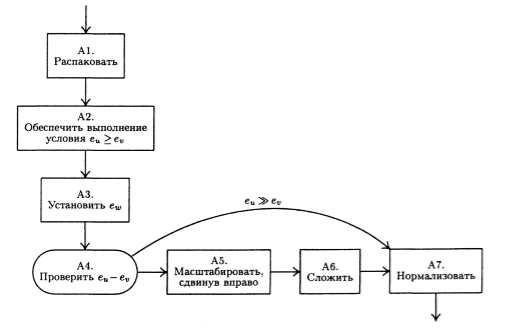
\includegraphics[scale=.9]{s}
\end{center}
\caption{Сложение чисел с плавающей точкой.}
\end{figure}


Первый (и наиболее трудный!) из алгоритмов, обсуждаемых в этом разделе, - это процедура сложения чисел с плавающей точкой:

\begin{equation}\label{f6}
(e_u,f_u) \oplus (e_v,f_v) = (e_w, f_w)
\end{equation}

\textit{Ввиду того что арифметические действия над числами с плавающей точкой являются по самой своей сути приближенными, а не точными, для обозначения операций сложения, вычитания, умножения и деления с плавающей точкой здесь будут использоваться ''округленные'' символы}
$$ \oplus, \ominus, \otimes, \oslash $$
\textit{чтобы отличать приближенные операции от точных.}

Идея, лежащая в основе сложения с плавающей точкой, довольно проста. Полагая, что $e_u \geqslant e_v$, формируем результат по принципу $e_w = e_u, f_w = f_u + f_v/b^{e_u-e_v}$ (таким образом, выравнивается положение разделяющих точек и соответственно положение разрядов слагаемых), а затем нормализуем результат. Может возникнуть несколько ситуаций, которые делают выполнение этого процесса нетривиальным; более точное описание метода дается в следующем алгоритме.

\subparagraph{Алгоритм А} (Сложение чисел с плавающей точкой). Для заданных p-разрядных нормализованных чисел с плавающей точкой $u = (e_u,f_u) и v = (e_v,f_v)$ по основанию b с избытком q строится сумма $\mu = u \oplus v$. Данный алгоритм (рис. 2) можно использовать и для вычитания чисел с плавающей точкой, если \textit{v} заменить на \textit{-v};.
\begin{enumerate}[label=A{\arabic*}]
\item\label{a1} [Распаковать.] Выделить порядок и дробную часть в представлениях для \textit{u} и \textit{v}.

\item\label{a2} [Обеспечить выполнение условия $e_u > e_v$] Если $е_u < e_v$, поменять местами \textit{u} и \textit{y}. (Во многих случаях удобнее совместить шаг \ref{a2} с шагом \ref{a1} или с каким-нибудь из последующих шагов.)

\item\label{a3} [Установить $e_w$] Установить $e_w \leqslant е_u$.

\item\label{a4} [Проверить $e_u - e_w$] Если $e_u - e_v > р + 2$ (большая разница в порядках), установить $f_w \leqslant f_u$ и перейти к шагу \ref{a7}. (Так как предполагается, что и нормализовано, на этом выполнение алгоритма можно было бы и закончить, но часто полезно использовать операцию сложения с нулем для гарантированной нормализации любого, возможно, и ненормализованного, числа.)

\item\label{a5} [Масштабировать, сдвинув вправо.] Сдвинуть $f_v$ вправо на $e_u - e_v$ позиций, т. е. разделить $f_v$ на $b^{e_u-ev}$. [\textit{Замечание.} Величина сдвига может достигать $р + 1$ разрядов, вследствие чего для выполнения следующего шага (сложения дробной части $f_u$ с $f_v$) потребуется аккумулятор, способный хранить $2р + 1$ цифр по основанию b справа от позиционной точки. Если такого вместительного аккумулятора нет, можно сократить сдвиг до $р + 2$ или $р + 3$ разрядов, но с соответствующими предосторожностями; подробности обсуждаются в упр. 5.]

\item\label{a6} [Сложить.] Установить $f_w \leftarrow f_u + f_v$.

\item\label{a7} [Нормализовать.] (В этот момент ($e_w,f_w$) представляет сумму $u$ и $w$, но $\mid f_w\mid$ может содержать более р цифр и может быть больше единицы или меньше 1/6.)Выполнить описываемый ниже алгоритм N, который нормализует и округлит $(z_w,f_w)'> а$ также сформирует окончательный результат.


\end{enumerate}


\subparagraph{Алгоритм N} (Нормализация). ''Грубый порядок'' $e$ и ''сырая дробная часть' f приводятся к нормализованному виду с округлением при необходимости до $p$ разрядов. В этом алгоритме (рис. 3) предполагается, что $|f| < b$.

\begin{enumerate}[label=N{\arabic*}]
\item\label{n1} [Проверить $f$.] Если $|f| \\geq 1/b$ (переполнение дробной части), перейти к шагу \ref{n4}. Если f = 0, установить e равным его наименьшему значению и перейти к шагу \ref{n7}.

\item\label{n2} [$f$ нормализовано?] Если $|f| > 1/b$, перейти к шагу N5.

\item\label{n3} [Масштабировать, сдвинув влево.] Сдвинуть $f$ на один разряд влево (т. е. умножить на b) и уменьшить $e$ на 1. Возвратиться к шагу \ref{n2}.

\item\label{n4} [Масштабировать, сдвинув вправо.] Сдвинуть $f$ вправо на один разряд (т. е. разделить на b) и увеличить $e$ на 1.

\item\label{n5} [Округлить.] Округлить $f$ до p разрядов: (Это означает, что / изменяется до ближайшего кратного $b^{-p}$. Возможно, что $(b^{p}f)$ mod 1 = $\frac{1}{2}$ т. е. имеется два ближайших кратных. Если $b$ четно, то заменяем $f$ ближайшим кратным $b^{-p}$, таким, что $b^{p}f' + \frac{1}{2}b$ нечетно (обозначим результат округления в таком случае через $f'$). Более подробное обсуждение аспектов округления приводится в разделе 4.2.2.) Важно отметить, что операция округления может привести к равенству $|f| = 1$ (переполнение при округлении); в такой ситуации следует вернуться к шагу \ref{n4}.

\item\label{n6} [Проверить e.] Если порядок $e$ слишком велик, т. е. больше допустимой границы, это воспринимается, как выполнение условия переполнения порядка. Если e слишком мал, это воспринимается, как выполнение условия исчезновения 
 
\begin{figure}

\begin{center}
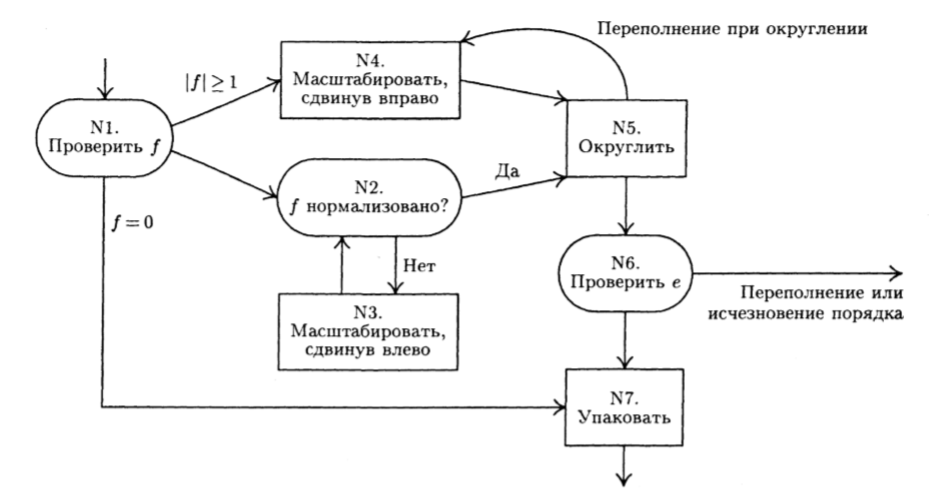
\includegraphics[scale=.6]{s2}
\end{center}
\caption{Нормализация $e$, $f$}
\end{figure}

порядка. (Дополнительная информация по этому вопросу приводится ниже; эти ситуации интерпретируются обычно, как сигнал об ошибке, в том смысле, что результат не может быть представлен в виде нормализованного числа с плавающей точкой из требуемого интервала значений.)

\item\label{n7} [Упаковать.] Объединить порядок $e$ и дробную часть $f$ для выдачи искомого результата.

Несколько простых примеров сложения чисел с плавающей точкой рассматривается в упр. 4.

Приведенные ниже подпрограммы для сложения и вычитания на компьютере MIX чисел, имеющих форму (\ref{f4}), служат примером программной реализации алгоритмов A и N. Эти подпрограммы извлекают одно входное значение и по символическому адресу ACC, другое входное значение $v$ извлекается из регистра A при входе в подпрограмму. Результат w одновременно появляется в регистре A поле ACC. Таким образом, последовательность команд

\begin{center}
\begin{equation}\label{f7}
\mathrm{LDA A;\quad ADD В;\quad SUB С;\quad STA D,}
\end{equation}
\end{center}
работающих с числами с фиксированной точкой, соответствовала бы такой последовательности команд, работающих с числами с плавающей точкой:
\begin{center}
\begin{equation}\label{f8}
\mathrm{LDA A,\quad STA АСС;\quad LDA В, JMP FADD;\quad LDA С, JMP FSUB;\quad STA D.}
\end{equation}
\end{center}

\end{enumerate}

\subparagraph{Программа А} \textit{(Сложение, вычитание и нормализация).} Следующая программа представляет собой подпрограмму, реализующую алгоритм A, причем она построена таким образом, что нормализующий фрагмент может использоваться другими 
подпрограммами, которые будут рассмотрены ниже. Как в этой программе, так и во многих других программах данной главы, идентификатор 0FL0 именует подпрограмму, которая печатает сообщение о том, что индикатор переполнения машины MIX внезапно перешел в состояние ''включено''. Предполагается, что размер байта b кратен 4. В подпрограмме нормализации NORM предполагается, что rI2 $= e$ и rAX $= f$, где rA $= 0$ влечет за собой rX $= 0$ и rI12 $< b$.

\begin{longtable}{l l l l l}
\textit{00}: & BYTE & EQU & 1(4:4) & Размер байта $b$.\\
\textit{01}: & EXP & EQU & 1:1 & Определение поля порядка.\\
\textit{02} & FSUB & STA & TEMP &	Подпрограмма вычитания чисел с плавающей точкой.\\
\textit{03} & & LDAN & TEMP & Изменить знак операнда.\\
\textit{04} & FADD & STJ & EXITF &	Подпрограмма сложения чисел с плавающей точкой.\\
\textit{05}	& & JOV & OFLO & Снятие блокировки переполнения.\\
\textit{06}	& & STA & TEMP & TEMP $\leftarrow v$.\\
\textit{07}	& & LDX & ACC & rX $\leftarrow u$\\
\textit{08}	& & CMPA & ACC(EXP)	& \underline{\textit{Шаги \ref{a1}-\ref{a3} скомбинированы ниже.}}\\
\textit{09}	& & JGE & 1F & Переход, если $e_v \geq e_u$.\\
\textit{10}	& & STX & FU(0:4) & FU $\leftarrow \pm f f f f 0$.\\

\textit{11}	& & LD2 & ACC(EXP) & rI2 $\leftarrow e_w$.\\
\textit{12}	& & STA & FV(0:4) &\\	
\textit{13}	& & LD1N & TEMP(EXP) & rI1 $\leftarrow -e_v$\\
\textit{14}	& & JMP & 4F &\\	
\textit{15} & 1H & STA & FU(0:4) & FU $\leftarrow \pm f f f f 0$ ($u$,$v$ меняются ролями).\\
\textit{16} & & LD2 & TEMP(EXP) & rI2 $\leftarrow e_w$.\\
\textit{17} & & STX & FV(0:4) &\\	
\textit{18}	& & LD1N & ACC(EXP) & rI1 $\leftarrow -e_v$.\\
\textit{19} & 4H & INC1 & 0,2 & rI1 $\leftarrow e_u - e_v$. (Шаг \ref{a4} не является необходимым.)\\
\textit{20} & 5H & LDA & FV & \underline{\textit{\ref{a5}. Масштабировать, сдвинув вправо.}}\\
\textit{21}	& & ENTX & 0 & Очистить rX.\\
\textit{22} & & SRAX & 0,1 & Сдвиг вправо на $e_u - e_v$ позиций.\\
\textit{23} & 6H & ADD & FU & \underline{\textit{\ref{a6}. Сложение.}}\\
\textit{24}	& & JOV & \ref{n4} & \underline{\textit{\ref{a7}. Нормализация.}} Переход, если произошло переполнение.\\
\textit{25}	& & JXZ & NORM & Простой случай?\\
\textit{26}	& & CMPA & =0=(1:1) & $f$ нормализовано?\\
\textit{27}	& & JNE & \ref{n5} & Если нормализовано, округлить его.\\
\textit{28}	& & SRC & 5 & |rX| $\leftrightarrow$ |rA|\\
\textit{29}	& & DECX & 1 & (rX положительно.)\\
\textit{30}	& & STA & TEMP & (Операнды имеют противоположные знаки;\\
\textit{31}	& & STA & HALF(0:0) & нужно уточнить состояние регистров\\
\textit{32}	& & LDAN & TEMP & перед округлением и нормализацией.)\\
\textit{33}	& & ADD & HALF &\\	
\textit{34}	& & ADD & HALF & Дополнить наименьшей значащей величиной.\\
\textit{35} & & SRC & 4 & Переход к подпрограмме нормализации.\\
\textit{36}	& & JMP & N3A & \\	
\textit{37} & HALF & CON & 1//2	& Половина размера слова (знак может изменяться).\\
\textit{38}	& FU & CON & 0 & Дробная часть $f_u$.\\
\textit{39} & FV & CON & 0 & Дробная часть $f_v$.\\
\textit{40}	& NORM & JAZ & ZRO & \underline{\textit{\ref{n1}. Проверить f.}}\\
\textit{41}	& \ref{n2} & СМРА	& =0=(1:1) & \underline{\textit{\ref{n2}. Нормализовано ли f?}}\\
\textit{42}	& & JNE & \ref{n5} & Перейти к шагу \ref{n5}, если ведущий байт отличен от нуля.\\
\textit{43} & \ref{n3} & SLAX & 1 & \underline{\textit{\ref{n3}. Масштабировать, сдвинув влево.}}\\
\textit{44}	& \ref{n3}A & DEC2 & 1 & Уменьшить $e$ на 1.\\
\textit{45}	& & JMP & \ref{n2} & Вернуться к шагу \ref{n2}.\\
\textit{46} & \ref{n4} & ENTX & 1 & \underline{\textit{\ref{n4}. Масштабировать, сдвинув вправо.}}\\
\textit{47}	& & SRC & 1 & Выполнить сдвиг вправо и вставить ''1'' с соответствующим знаком.\\
\textit{48}	& & INC2 & 1 & Увеличить $e$ на 1.\\
\textit{49} & \ref{n5}& СМРА & =BYTE/2=(5:5) & \underline{\textit{\ref{n5}. Округление.}}\\
\textit{50}	& & JL & \ref{n6} & |остаток| $< \frac{1}{2}b$?\\
\textit{51}	& & JG & 5F &\\	
\textit{52}	& & JXNZ & 5F & |остаток| $> \frac{1}{2}b$?\\
\textit{53}	& & STA & TEMP & |остаток| = $\frac{1}{2}b$; округлить до нечетного\\
\textit{54}	& & LDX & TEMP(4:4) &\\	
\textit{55}	& &	JX0 & N6 & Перейти к шагу \ref{n6}, если rX нечетно.\\
\textit{56} & 5Н & STA & *+1(0:0) & Сохранить знак rA.\\
\textit{57}	& & INCA & BYTE & Добавить $b^{-4} $ к |f| (знак может изменяться).\\
\textit{58} & & J0V & N4 & Проверить переполнение и-за округления.\\
\textit{59} & N6 & J2N & EXPUN & \underline{\textit{\ref{n6}. Проверка $e$.}} Исчезновение порядка, если $e < 0$.\\
\textit{60}	& \ref{n7} & ENTX & 0,2 & \underline{\textit{\ref{n7}. Упаковать.}} rX $\leftarrow e$.\\
\textit{61} & & SRC & 1 &\\	
\textit{62}	& ZR0 & DEC2 & BYTE & rI2 $\leftarrow e - b$.\\
\textit{63} & 8Н & STA & ACC &\\
\textit{64} & EXITF & J2N & * & Выход, если только не $e \geq b$.\\
\textit{65} & EXP0V & HLT & 2 & Обнаружено переполнение порядка.\\
\textit{66}	& EXPUN & HLT & 1 & Обнаружено исчезновение порядка.\\
\textit{67}	& АСС & CON	& 0 & Аккумулятор для операций с плавающей точкой.\\

\end{longtable}

Довольно большой фрагмент кода программы (строки 25-37) включен в программу по той причине, что в MIX имеется 5-байтовый аккумулятор для сложения чисел со знаком, в то время как алгоритм A в общем случае требует для него $2p + 1 = 9$ разрядов. В действительности всю программу можно сократить почти вдвое, если пожертвовать хотя бы небольшой долей точности. Однако, как будет показано в следующем разделе, всегда лучше получать наибольшую возможную точность. В строке 55 используется нестандартная команда MIX, описанная в разделе 4.5.2. Время выполнения сложения и вычитания чисел с плавающей точкой зависит от нескольких факторов, анализируемых ниже, в разделе 4.2.4.

Рассмотрим теперь операции умножения и деления, которые выполняются проще, чем сложение, и довольно похожи одна на другую.

\subparagraph{Алгоритм М} \textit{(Умножение или деление чисел с плавающей точкой).} По данным р-разрядным нормализованным числам с плавающей точкой $u = (e_u,f_u)$ и $v = (e_v, f_v)$ по основанию $b$ с избытком $q$ строится произведение $w = u \otimes v$ или частное
$w = u \oslash v$
\begin{enumerate}[label=M{\arabic*}]
\item\label{m1} [Распаковать.] Выделить порядки и дробные части в представлениях $u$ и $v$

\noindent(Иногда удобно, хотя и необязательно, проверить в ходе выполнения этого шага, не равны ли операнды нулю.)

\item\label{m2} [Выполнить операцию.] Установить

%\begin{equation}
%\begin{array}{c}
%\text{\begin{tabular}{lll}
%\\
%\end{tabular}}
%
%\end{array}
%\end{equation}

\begin{equation}\label{f9}
\begin{array}{lll} 
e_w \leftarrow e_u + e_v - q, & f_w \leftarrow f_u f_v &\text{для умножения;}\\ 
e_w \leftarrow e_u - e_v + q + 1, &f_w \leftarrow (b^{-1}f_u)/f_v &\text{для деления.}\\

\end{array} 
\end{equation}

(Поскольку предполагается, что вводимые числа нормализованы, в результате получим, что либо $f_w - 0$, $либо 1/b^2 \leq |f_w| < 1$, либо возникнет ошибка ''деление на нуль''.) Здесь, если в этом есть необходимость, можно урезать $f_w$ до $p + 2$ или $p + 3$ разрядов, как в упр. 5.

\item\label{m3} [Нормализовать.] Применить к $(e_w,f_w)$ алгоритм N с тем, чтобы нормализовать, округлить и упаковать результат. (\textit{Замечание.} В этом случае нормализация выполняется проще ввиду того, что масштабирование посредством сдвига влево происходит не более одного раза и после деления переполнение не может возникнуть вследствие округления.)
\end{enumerate}
В подпрограммах для MIX, тексты которых приведены ниже, используются те же соглашения, что и в программе А. Эти подпрограммы служат примером машинной реализации алгоритма М.

\textbf{Программа M.} \textit{(Умножение и деление чисел с плавающей точкой).}
\begin{longtable}{l l l l l}
\textit{01} & Q & EQV & BYTE/2 & $q$ есть половина байта.\\
\textit{02} & FMUL & STJ & EXITF & Подпрограмма умножения чисел с плавающей точкой.\\
\textit{03} &  & J0V & 0FL0 & Снятие блокировки переполнения.\\
\textit{04} &  & STA & TEMP & TEMP $\leftarrow v$.\\
\textit{05} &  & LDX & ACC & rX $\leftarrow v$\\
\textit{06} &  & STX & FU(0:4) & FU $\leftarrow \pm f f f f 0$.\\
\textit{07} &  & LD1 & TEMP(EXP) &\\
\textit{08} &  & LD2 & ACC(EXP) &\\
\textit{09} &  & INC2 & -Q,l & rI2 $\leftarrow e_u + e_v - q$\\
\textit{10} &  & SLA & 1 &\\
\textit{11} &  & MUL & FU & Умножить $f_u$ на $f_v$.\\
\textit{12} &  & JMP & NORM & Нормализовать, округлить и выйти из подпрограммы.\\
\textit{13} & FDIV & STJ & EXITF & Подпрограмма деления чисел с плавающей точкой.\\
\textit{14} &  & J0V & OFLO & Снятие блокировки переполнения.\\
\textit{15} &  & STA & TEMP & TEMP $\leftarrow v$.\\
\textit{16} &  & STA & FV(0:4) & FV $\leftarrow \pm f f f f 0 $.\\
\textit{17} &  & LD1 & TEMP(EXP) &\\
\textit{18} &  & LD2 & ACC(EXP) &\\
\textit{19} &  & DEC2 & -Q,l & rI2 $\leftarrow e_u - e_v + q$.\\
\textit{20} &  & ENTX & 0 &\\
\textit{21} &  & LDA & ACC &\\
\textit{22} &  & SLA & 1 & rA $\leftarrow f_u$.\\
\textit{23} &  & СМРА & FV(1:5) &\\
\textit{24} &  & JL & *+3 & Переход, если $|f_u| < |f_v|$.\\
\textit{25} &  & SRA & 1 & Иначе - масштабировать $f_u$ вправо\\
\textit{26} &  & INC2 & 1 & и увеличить rI2 на 1.
\end{longtable}

Наиболее интересная особенность этой программы - подготовка к выполнению деления, осуществляемая командами в строках 23-26. Эти операции проводятся для того, чтобы обеспечить достаточную точность при округлении ответа. При $|f_u| < |f_v|$, непосредственно применив алгоритм M, можно сохранить результат в форме ''$\pm 0 f f f f$'' в регистре А, что сделает невозможным чистое округление без специального анализа остатка (он хранится в регистре X). Поэтому в такой ситуации программа вычисляет $f_w \leftarrow f_u / f_v$, гарантируя, что $f_w$ либо равно нулю, либо во всех случаях нормализовано. Процедура округления может оперировать пятью значащими байтами, возможно, проверяя, не равен ли остаток нулю.

Иногда может потребоваться перевод из представления с фиксированной точкой в представление с плавающей точкой и обратно. При помощи описанного выше алгоритма нормализации легко получается программа перевода ''из фиксированной в плавающую''. Например, целое число переводится в форму с плавающей точкой с помощью следующей подпрограммы на языке MIX.

\begin{equation}\label{FLOT}
\begin{array}{l l l l l} 
\textit{01} & \text{FLOT STJ} & \text{EXITF} & \text{Предполагаем, что rA} = u \; \text{есть целое число.}\\
\textit{02} & \text{J0V} & \text{0FL0} & \text{Снятие блокировки переполнения.}\\
\textit{03} & \text{ENT2} & \text{Q+5} & \text{Установить ''грубый'' порядок.}\\
\textit{04} & \text{ENTX} & 0 &\\
\textit{05} & \text{JMP} & \text{NORM} & \text{Нормализовать, округлить и выйти из подпрограммы.}\\
\end{array}
\end{equation}

\noindent Подпрограмма перевода ''из плавающей в фиксированную'' служит предметом упр. 14.

Отладка подпрограмм выполнения арифметических операций над числами с плавающей точкой - обычно довольно сложная задача из-за обилия различных случаев, которые нужно предусмотреть. Ниже перечислены распространенные ловушки, подстерегающие программиста, который занимается программами ''плавающей арифметики''.

\begin{enumerate}
\item[1)] \textit{Потеря знака.} Во многих машинах (к MIX это не относится) команды сдвига регистров воздействуют на знаковый разряд, поэтому следует подробно анализировать операции сдвига, используемые при нормализации и изменении масштаба дробной части числа. Часто знак теряется и при появлении ''минус нуля''. (Например, операторы 30-34 программы A ответственны за установку знакового разряда регистра А. См. также упр. 6.)

\item[2)] \textit{Невозможность правильного определения, что произошло - исчезновение или переполнение порядка.} Не следует проверять величину $e_w$ до окончания операций округления и нормализации, так как предварительные проверки могут привести к ошибочным результатам. Исчезновение и переполнение порядка могут происходить и при выполнении сложения и вычитания, а не только при умножении и делении, и, несмотря на то что это событие довольно редкое, проверку необходимо проводить для каждого конкретного случая. Для того чтобы выполнить необходимые корректирующие операции после обнаружения исчезновения или переполнения, нужно заранее позаботиться о сохранении достаточной для этого информации.

К сожалению, некоторые программисты во многих случаях пренебрегают исчезновением порядка. Они просто полагают, что исчезающе малые результаты равны нулю без индикации ошибки. Часто это приводит к серьезной потере точности (а на самом деле к потере \textit{всех} значащих цифр), что нарушает соглашения, принятые в операциях над числами с плавающей точкой. Таким образом, системная подпрограмма действительно должна информировать прикладного программиста об исчезновении порядка. Приравнивание результата к нулю допустимо только в отдельных случаях, когда результат должен складываться со значительно большей величиной. Если исчезновение порядка не фиксируется, то возникают таинственные ситуации, когда $(u \otimes v) \otimes w$ равно нулю, а $u \otimes (v \otimes w)$ нет, поскольку, скажем, умножение и $u \otimes v$ приводит к исчезновению порядка, а $u \otimes ( v \otimes w)$ вычисляется и без выхода порядков за пределы допустимого интервала. Подобным же образом можно найти пять таких положительных чисел $a,b,c,d$ и $y$, что
\begin{equation} \label{q1}
\begin{array}{c} 
(a \otimes y \otimes b ) \oslash (c \otimes y \oplus d) \approx \frac{2}{3}\\
(a \oplus b \oslash y) \oslash (c \oplus d \oslash y) = 1\\
\end{array}
\end{equation}

если исчезновение порядка не фиксируется (см. упр. 9). Даже с учетом того, что подпрограммы арифметики с плавающей точкой не идеально точны, такие несуразные результаты, как (\ref{q1}), совсем уж неожиданны для случая, когда все числа $a,b,c,d$ и $y$ \textit{положительны!} Исчезновение порядка обычно не предугадывается программистом, так что ему следует об этом сообщать *.

\item[3)] \textit{Попадание ''мусора''.} При выполнении сдвига влево необходимо проследить, чтобы в освобождающиеся разряды справа не было введено чего-либо, отличного от нулей. Например, обратите внимание на команду ENTX 0 в строке 21 программы А и ''слишком легко забываемую'' команду ENTX 0 в строке 04 подпрограммы FL0T в (\ref{FLOT}). (Но было бы ошибкой очищать регистр X после строки 27 в подпрограмме деления.)

\item[4)] \textit{Непредусмотренное переполнение при округлении.} Когда число наподобие .999999997 округляется до 8 цифр, происходит перенос влево от десятичной точки и результат сдвигается вправо. Многие ошибочно считали, что в ходе выполнения

\footnote{С другой стороны, нужно отметить, что современные языки программирования высокого уровня предоставляют программисту (или вовсе не предоставляют) весьма ограниченные возможности использования информации, содержащейся в стандартных программах арифметики с плавающей точкой. Подпрограммы для MIX, которые представлены в этом разделе, просто останавливают работу, обнаружив такую ситуацию, а это отнюдь не выход. Существует множество приложений, для которых исчезновение порядка относительно безвредно, и потому желательно найти способ, пользуясь которым программист смог бы просто и безопасно для приложения справиться с возникшей проблемой. Практика подстановки ''втихомолку'' нуля вместо результата с исчезнувшим порядком себя полностью дискредитировала, но существует альтернатива, которая в последнее время завоевывает все большую популярность. Ее суть в том, чтобы модифицировать самое определение формата представления чисел с плавающей точкой, допуская существование ненормализованной дробной части в случае, если порядок имеет минимальное допустимое значение. Эта идея ''постепенной потери значимости'' впервые была реализована в компьютере Electrologica Х8; она лишь незначительно усложнила алгоритмы выполнения операций, но совершенно исключила возможность исчезновения порядка при сложении и вычитании. Рассмотрение этой идеи выходит за рамки данной книги, поэтому в простых формулах анализа относительной ошибки вычислений в разделе 4.2.2 появление постепенной потери значимости не учитывается. Тем не менее, используя формулы, подобные $\text{round}(x)= x(1 - \delta) + e, \text{где} |\delta | < b^{1-p}/2 \text{и} |e| < b^{-p-q}/2$, можно показать, что формат с постепенной потерей значимости успешно срабатывает во многих важных случаях. (См. W. М. Kahan and J. Palmer, ACM SIGNUM Newsletter (October, 1979), 13-21.)}
умножения переполнение при округлении невозможно, так как максимальное значение $|f_{u}f_{w}|$ равно $1- 2b^{-p} + b^{-2p}$, а это число не может округлиться до 1. Ошибочность такого рассуждения продемонстрирована в упр. 11. Любопытно, что переполнение при округлении действительно невозможно при делении чисел с плавающей точкой (см. упр. 12).

Существует направление, представители которого утверждают, что можно безболезненно ''округлять'' .999999997 до .99999999, а не до 1.0000000, поскольку последний результат представляет все числа из интервала
\begin{center}
$[1.0000000 - 5 \times 10^{-8} .. 1.0000000 + \times 10^{-8}$,
\end{center}
в то время как .99999999 представляет все числа из гораздо меньшего интервала
\begin{center} 
$(.99999999 - 5 \times 10^{9} .. .99999999 + 5 \times 10^{-9}$.
\end{center}
Хотя второй интервал и не содержит исходного числа .999999997, каждое число из второго интервала содержится в первом, так что последующие вычисления со вторым интервалом не менее точны, чем с первым. Но этот довод несовместим с математической идеологией арифметики с плавающей точкой, представленной ниже, в разделе 4.2.2.
 
\item[5)] \textit{Округление до нормализации.} Неточность результата порождается и преждевременным округлением в неверных цифровых разрядах. Эта ошибка очевидна, когда округление производится слева от соответствующего разряда. Она также опасна в менее очевидном случае, когда округление сначала выполняется намного правее, а затем - в истинном разряде. По этой причине ошибочно осуществлять округление в ходе операции ''сдвиг вправо'' на шаге A5; исключением является случай, рассмотренный в упр. 5. (Однако специальный случай округления на шаге N5, а затем повторного округления уже после переполнения при округлении безобиден, потому что переполнение при округлении всегда приводит к значению $\pm 1.0000000$, которое не меняется в результате последующей процедуры округления.)

\item[6)] \textit{Невозможность сохранения достаточной точности в промежуточных вы-числениях.} Детальный анализ точности арифметических операций с плавающей точкой, проводимый в следующем разделе, показывает, что нормализующие программы арифметики с плавающей точкой должны всегда обеспечивать максимальную точность подходящим образом округленного результата. Не должно быть никаких отступлений от этого принципа, даже в тех случаях, появление которых предельно маловероятно. Надлежащее число значащих цифр следует сохранять в ходе всех промежуточных вычислений, как реализовано в алгоритмах А и М.
\end{enumerate}

\subparagraph{С. Аппаратная реализация арифметических действия над числами с плавающей точкой.} В арсенале почти каждой большой ЭВМ, предназначенной для научных расчетов, содержатся встроенные операции и команды арифметических операций над числами с плавающей точкой. К несчастью, в аппаратных реализациях таких команд обычно присутствуют некоторые дефекты, приводящие при определенных обстоятельствах к удручающе скверному поведению машины, и, надо надеяться, в будущем создатели вычислительной техники будут уделять больше внимания данному вопросу. Затраты на это очень малы, и соображения, представленные в следующем разделе, показывают, какой выигрыш может быть достигнут. Из того, что сегодня известно, следует, что для современных компьютеров не подходят вчерашние компромиссные решения.
Компьютер MIX, используемый в этой серии книг как пример ''типичной'' вычислительной машины, оснащается средством расширения для работы с числами в формате с плавающей точкой - арифметическим расширителем. Он доступен за небольшую дополнительную сумму и обеспечивает выполнение следующих шести команд на аппаратном уровне.

\point{} FADD, FSUB, FMUI, FDIV, FLOT, FCMP (C = 1, 2, 3, 4, 5, 56 соответственно; F=6). Содержимое регистра rA после выполнения команды FADD V такое же, как и содержимое rA после выполнения команд
\begin{center}
STA ACC; LDA V; JMP FADD.
\end{center}

Здесь FADD - подпрограмма, которая уже появлялась выше в этом разделе, но оба операнда автоматически нормализуются непосредственно перед входом в подпрограмму, если они еще не были нормализованы. (Если во время предварительной нормализации, но не во время нормализации результата, возникает исчезновение порядка, вызывающая программа о нем не извещается.) Аналогичные замечания относятся к операциям FSUB, FMUL и FDIV. Содержимое регистра rA после выполнения операции FL0T совпадает с его же содержимым после выполнения команды JMP FL0T в подпрограмме (\ref{FLOT}). Содержимое rA не искажается командой FCMP V. Эта команда устанавливает индикатор сравнения в состояние LESS, EQUAL или GREATER в зависимости от того, будет ли содержимое rA ''заметно меньше, чем'', ''примерно равно'' или ''заметно больше, чем'' V, как обсуждается в следующем разделе. Работа этой команды в точности моделируется подпрограммой FCMP из упр. 4.2.2-17 с EPSILON в ячейке 0.

Ни одна из команд арифметики с плавающей точкой не воздействует ни на какой другой регистр, помимо rA. Если происходит переполнение или исчезновение порядка, то включается индикатор переполнения и указывается порядок результата по модулю размера байта. Попытка деления на нуль оставляет в регистре rA ''мусор'' (произвольное значение). Времена выполнения: $4u, 4u, 9u, 11u, 3u$ и $4u$ соответственно.

\point{} FIX (С = 5; F = 7). Содержимое rA заменяется целым числом ''round(rA)'', округленным до ближайшего целого, как на шаге N5 алгоритма N. Однако, если этот результат слишком велик и не вмещается в разрядную сетку регистра, устанавливается индикатор переполнения и результат должен трактоваться как неопределенный. Время выполнения: $3u$.

Иногда полезно использовать операторы арифметики с плавающей точкой нестандартным образом. Например, если бы операция FL0T не была реализована как часть арифметического расширителя компьютера MIX, можно было бы легко обеспечить ее выполнение для 4-байтовых чисел, написав маленькую подпрограмму

\begin{equation}\label{FLAT}
\begin{array}{l l l} 
\text{FLOT} & \text{STJ} & \text{9F}\\
& \text{SLA} & 1\\
& \text{ENTIX} & \text{Q+4}\\
& \text{SRC} & 1\\
& \text{FADD} & \text{=0=}\\
9H & \text{JMP} & \text{*}\\
\end{array}
\end{equation}

Эта программа не эквивалентна команде FL0T, так как в ней предполагается, что 1:1 байт регистра rA равен нулю; кроме того, она портит содержимое регистра rX.

В более общих ситуациях приходится прибегать ко всяким хитростям, потому что переполнение при округлении может происходить даже во время выполнения команды FL0T.

Аналогично предположим, что MIX имеет команду FADD, но не имеет FIX. Чтобы округлить число и. записанное в формате с плавающей точкой, до ближайшего целого числа с фиксированной точкой (причем известно, что число неотрицательно и займет не более трех байтов), в программе можно записать
\begin{center}
FADD FUDGE,
\end{center}
где в ячейке FUDGE содержится константа

\begin{center}
\begin{tabular}{|l|l|l|l|l|l|}
\hline +&Q+4&1&0&0&0\\\hline
\end{tabular}
\end{center}

результат в rA будет иметь вид

%\begin{equation}\label{rez}
%\begin{array}{c}
%\text{\begin{tabular}{|l|l|l|l|l|l|}
%\hline +&\text{Q+4}&1&\text{Округлённое}(u)\\\hline
%\end{tabular}} 
%\end{array}.
%\end{equation}

\begin{equation}\label{rez} 
\bitpattern[noBitNumbers]{+}[1]{Q+4}[3]{1}[1]{Округленное}[9]/ 
\end{equation}

\subparagraph{D. История и библиография.} Истоки арифметики чисел с плавающей точкой прослеживаются вплоть до вавилонян (около 1800 г. до н. э. или ранее), которые применяли арифметические операции над числами с плавающей точкой по основанию 60, но не имели обозначения для порядка. Нужный порядок всегда некоторым образом ''подразумевался'' тем, кто производил вычисления. По крайней мере в одном случае обнаружено, что у вавилонян получился ошибочный ответ, потому что сложение осуществлялось при неверно выполненном выравнивании операндов, однако это случалось весьма редко (см. О. Neugebauer, The Exact Sciences in Antiquity (Princeton, N. J.: Princeton University Press, 1952), 26-27). Другой пример раннего обращения к формату с плавающей точкой связан с именем греческого математика Аполлония (3 в. до н. э.), который, повидимому, был первым, кто объяснил, как можно упростить умножение, по крайней мере в простых случаях, собирая степени 10 отдельно от их коэффициентов. Метод Аполлония обсуждается в труде Паппа Александрийского ''Математическое собрание'' (4 в. н. э.). После гибели вавилонской цивилизации представление с плавающей точкой существенным образом использовалось для формирования произведений и частных лишь много веков спустя, когда были открыты логарифмы (1600 г.) и вскоре после этого Отред (Oughtred) изобрел логарифмическую линейку (1630 г.). Примерно в тот же период было введено современное обозначение ''$x^n$'' для порядков; отдельные символы для квадрата х, куба x ит. д. - использовались и раньше.

Арифметика с плавающей точкой была включена в конструкцию некоторых из самых ранних вычислительных машин. Это было независимо предложено Леонардо Торресом-и-Овьедо (Leonardo Torres у Quevedo) в Мадриде (1914 г.), Конрадом Цузе (Konrad Zuse) в Берлине (1936 г.) и Джорджем Стибицем (George Stibitz) в Нью-Джерси (1939 г.). В машине Цузе использовалось двоичное представление с плавающей точкой, которое он назвал полулогарифмической нотацией; он также реализовал соглашение относительно операций с некоторыми особыми величинами, подобными ''$\infty$'' и ''не определено''. Первой американской вычислительной машиной, в которой появились средства для выполнения операций в формате с плавающей точкой, была Модель V (Bell Laboratories), за которой последовала гарвардская машина Марк II. Обе эти машины, спроектированные в 1944 году,

\end{document}